\section{Problem Formulation}
\label{sec:problem}
The event video localization task is to retrieve environment images from database given the query event video. 
The database images are automatically downloaded from online map service given a circle or rectangle shaped district where the event happened. 
If the video is taken on the ground, the database images will be Google street view images;
if the video is taken from a 45 degree up to down perspective of view, the database images will be Google satellite images. 
The details of database image generation will be elaborated in section~\ref{sec:solution}. 

A query video is composed of frames $\{q\}$. 
As we process one frame per time in matching the database, we abbreviate one frame from the query video as query for the ease of representation. 
The environment image from the database is denoted as $d$ and the database is denoted as $D = \{d\}$. 
We divide images into a three-level spatial pyramid of regions: $1 \times 1$, $2 \times 2$, $3 \times 3$ as shown in Figure~\ref{fig:regions}. 
We assign each region a saliency score $s$ to indicate how import the region is in matching. 
Please refer to Section~\ref{sec:expr} for region division details. 
We use subscript to represent region index. 
That is, we have saliency score $s(q_i)$ for region $i$ in query $q$ and $s(d_j)$ for region $j$ in the database image $d$. 
We define the non-negative matching score between two regions as $m(q_i, d_j; \mathbf{\Theta})$, where $\mathbf{\Theta}$ is the parameters to be learn. The similarity of two regions is proportional to their matching score.
For the ease of notation, we will use $m(q_i, d_j; \mathbf{\Theta})$ and $m(q_i, d_j)$ interchangeably in the following. 
\begin{figure}[htbp]
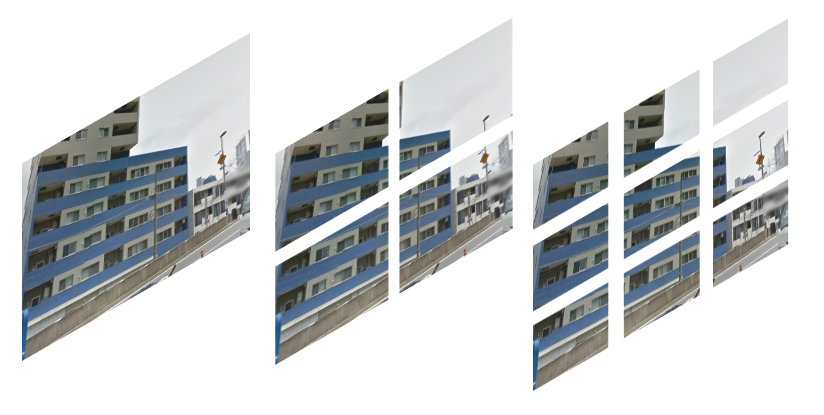
\includegraphics[width=0.8\linewidth]{img/regions}
\caption{The regions of an image}
\label{fig:regions}
\end{figure}

Now we have defined regions in the image, saliency score on regions and matching score between regions. 
Putting all these together, we define the matching score between query and database image as weighted sum of region matching scores:
\small
\begin{align}
\label{eq:img_match}
M(q, d) &= \sum_{i, j} w_{ij}\, m(q_i, d_j)\\
\label{eq:weight}
w_{ij} &= s(q_i) + s(d_j)
\end{align}
\normalsize
where the weight $w_{ij}$ is defined as the sum of saliency score of both regions. 
On the one hand, if both regions are salient and their matching score is high, such region pair contribute much to the final matching score $M(q, d)$. 
On the other hand, even if the matching score between two regions is high, but if both regions are not salient (e.g. road or tree), such region pair doesn't contribute much to the final matching score $M(q, d)$. 
% In the test stage, we assign the location of the query by averaging GPS location of top $K$ retrieved environment images. 

In the training stage, we automatically generate the labels of image pairs from database $D$ by leveraging the GPS information assigned to each environment image. 
The label $y_{(q, d)}$ of image $q$ and $d$ is $1$ if two images are matched and $0$ vice versa. 
The training data is denoted as: 
\small
\begin{equation}
\begin{aligned}
D_{train} &= \{(q, d, y_{(q, d)})\}\\
q &\in D, d \in D
\end{aligned}
\end{equation}
\normalsize
The details of automatically generating $D_{train}$ from $D$ are given in section~\ref{sec:solution}. 
Note that the labels are given on image pairs rather than region pairs. 
As the matching model $m(q_i, d_j; \mathbf{\Theta})$ is defined on region pair, the labels are actually weak labels. 
We use contrastive noise loss function as $L(q, d, y)$:
\small
\begin{equation}
\label{eq:img_loss}
\begin{aligned}
L(q, d, y) &= L_P(q, d, y) + L_N(q, d, y) \\
L_P(q, d, y) &= -y\sum_{y_{(q, d)}=1} M(q, d)\\
L_N(q, d, y) &= -(1-y)\sum_{y_{(q, d)}=0} \max(0, \Delta-M(q,d))
\end{aligned}
\end{equation}
\normalsize
where $\Delta$ is a hyper-parameter to keep unmatched pairs having small matching scores, $L_P$ is the loss function for matched pairs, $L_N$ is the loss function for unmatched pairs. 
We use eq~\eqref{eq:img_match} to expand image matching $M(q, d)$ term in the loss function:
\small
\begin{equation}
\label{eq:region_loss}
\begin{aligned}
L(q, d, y) = &-y\sum_{y_{(q, d)}=1} M(q, d) - (1-y) \sum_{y_{(q, d)}=0} \max(0, \Delta - M(q, d))\\
= & -y\, \sum_{i, j}\sum_{y_{(q, d)}=1} w_{ij}\, m(q_i, d_j) \\
 &- (1-y)\, \sum_{i, j}\sum_{y_{(q, d)}=0} w_{ij}\, \max(0, \Delta^{'} - m(q_i, d_j))\\
= & \underbrace{\sum_{i, j} w_{ij}\, L_P(q_i, d_j)}_{L_P(q, d)} + \underbrace{\sum_{i,j} w_{ij}\, L_N(q_i, d_j)}_{L_N(q, d)}
\end{aligned}
\end{equation}
\normalsize
In the last step substitution, we denote
\small
\begin{equation}
\label{eq:correspondence}
\begin{aligned}
L_P(q_i, d_j, y) &= -y\sum_{i,j}\sum_{y_{(q, d)}=1} m(q_i, d_j)\\
L_N(q_i, d_j, y) &= -(1-y)\sum_{i,j}\sum_{y_{(q, d)}=0} \max(0, \Delta^{'} - m(q_i, d_j))
\end{aligned}
\end{equation}
\normalsize
The last step in eq~\eqref{eq:correspondence} shows that the two components in image level loss, $L_P(q, d, y)$ and $L_N(q, d, y)$, are weighted sum of the two components in region level loss, $L_P(q_i, d_j, y)$ and $L_N(q_i, d_j, y)$, respectively. 
Furthermore, if we consider the region level label to be the same as its corresponding image level label, i.e. $y_{(q_i, d_j)} = y_{(q, d)}$, we could see that region level loss $L_P(q_i, d_j, y)$, $L_N(q_i, d_j, y)$ in eq~\eqref{eq:region_loss} has exactly the same form of image level loss $L_P(q, d, y)$, $L_N(q, d, y)$ in eq~\eqref{eq:img_loss}. 
However, recall that the major challenge in event video localization, large appearance change, leads to the fact that $y_{(q,d)} = 1$ doesn't imply that $y_{(q_i, d_j)} = 1, \forall q_i \in q, \forall d_j \in d$. 
In our problem formulation, we solve this issue by multiplying a region pair dependent weight $w_{ij}$ to each region level loss $L_P(q_i, d_j)$. 
Note that $w_{ij}$ is defined by saliency $s(q_i)$ and $s(d_j)$. 
That is, we could suppress the influence of ``wrong'' region level label to the final loss function through saliency. 

We recap all the above deduction into one main problem. 
\small
\begin{equation*}
\begin{aligned}
\text{main problem:}\\
min_{\mathbf{S}, \mathbf{\Theta}} L(q, d, y; \mathbf{S}, \mathbf{\Theta}) &= -y\, \sum_{i, j}\sum_{y_{(q, d)}=1} w_{ij}\, m(q_i, d_j; \mathbf{\Theta}) \\
& - (1-y)\, \sum_{i, j}\sum_{y_{(q, d)}=0} w_{ij}\, \max(\Delta^{'}-m(q_i, d_j; \mathbf{\Theta}))\\
w_{ij} &= s(q_i) + s(d_j)\\
% \mathbf{S} &= \{s(q_i)\} \cup \{s(d_j)\}\\  
s.t. & ||s(q)||_2 = 1 \quad \forall q\\
& ||s(d)||_2 = 1 \quad \forall d\\
& s(q_i), s(d_j) \in [0,1] \\
& y\in \{+1, 0\}
\end{aligned}
\end{equation*}
\normalsize
The notations introduced in this section are summarized in table~\ref{table:notations}. 

\begin{table}[htbp]
\begin{center}
\begin{tabular}{|c|p{0.35\textwidth}|}
\hline
$q_i$ & region $i$ in the query image $q$\\[0.2cm]
$d_j$ & region $j$ in the database image $d$\\[0.2cm]
$s(q_i), s(d_j)$ & the saliency of the region $q_i, d_j$ \\[0.2cm]
$m(q_i, d_j)$ & non-negative matching score between region $q_i$ and $d_j$ \\[0.2cm]
% $Q$ & all video frames $\{q\}$ \\[0.2cm]
% $D$ & all database images $\{d\}$ \\[0.2cm]
\hline
\end{tabular}
\end{center}
\caption{Notations introduced in this section.}
\label{table:notations}
\end{table}
